%Intro to intro
This thesis examines the opportunity and possibility to connect an embedded IoT device to a local Eclipse Arrowhead framework cloud.
This project uses the STM32 B-L4S5I-IOT01A IoT discovery node as a development board, running the Mbed-OS 6. 
\section{Background}
%Setting
According to Artemis-IA, the world is undergoing a new industrial revolution, moving towards a more decentralized and software-oriented means of production\cite{Artemis2021}.
This fourth new, and in some sense planned, industrial revolution is called Industry 4.0 according to Lasi\cite{Lasi2014}. 
%Technologies
Cyber-Physical systems act as a bridge between the data-rich cybernetic world and the technology-rich physical world Artemis-IA means\cite{Artemis2021}.
Artemis-IA claims that a differentiating factor between traditional embedded systems and Cyber-Physical systems is their size and scope, where traditional embedded systems have a more limited capacity.
Cyber-Physical system, on the other hand, has a much larger scope, including interconnected embedded systems, human-, and socio-technological systems as well Artemis-IA adds.

%Economic incentives.  
The larger economies of the world all have incentives promoting Industry 4.0, for instance, China’s Made in China 2025,
If Europe is to compete with the larger economies,  Europe needs to invest in the technologies mentioned above according to Artemis-IA\cite{Artemis2021}.
A shift away from proprietary solutions towards collaborative solutions  Artemis-IA claim need to happen in their report Embedded intelligence. 

\section{Motivation}
%Solve problem presented in the background.
The need for a European incentive promoting Industry 4.0 is clear. 
According to their website, the Arrowhead Tools project aims for digitalization and automation solutions for the European industries\cite{AT2021}.
The Arrowhead Tools project uses the open-source Eclipse Arrowhead framework, further contributing to the collaborative solutions needed for the European economy defined in the previous section.

%What is there now?
The Eclipse Arrowhead framework contains many examples in various programming languages.
Python, C\#, and C++ have client libraries and example code developed for them, which you can find on the project’s GitHub page.\cite{AC2021} 

%What is needed?
However, there is no client library or code example for a specific piece of hardware to connect to a local Arrowhead cloud fast and easy, showcasing the capabilities of this project. 
Therefore, a project with the clear intent to showcase both the capabilities and possibilities of Cyber-Physical systems and the Eclipse Arrowhead framework is needed.

%Conclussion to motivation
This thesis examines the possibilities of having a ready-made example to compile and run on a specific hardware platform that connects a local Arrowhead cloud as a proof of concept. 
Much like the ‘Getting started with’ examples from Amazon Web Services and Microsoft Azure.\cite{Guide2020,AZURE2021}
\section{Problem definition}
%This is good; if deleting the other paragraph, expand this.
This project aims to investigate the possibilities, benefits, and limitations of using the Eclipse Arrowhead framework on embedded devices in contrast to commercially available solutions such
as Amazon’s Amazon Web Services and Microsoft Azure. 
\begin{figure}[h!]
    \centering
    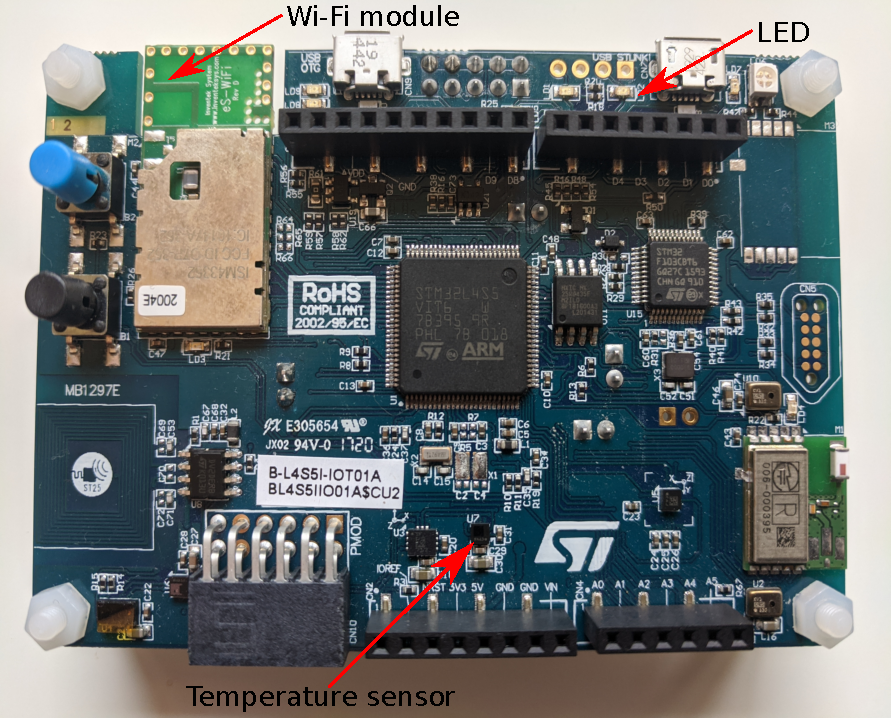
\includegraphics[width=\textwidth, height=10cm]{Pictures/board.pdf} 
    \caption{STM32 B-L4S5I-IOT01A IoT discovery node with relevant sensors and modules.}
    \label{STM32 B-L4S5I-IOT01A IoT discovery node}
\end{figure}
This thesis 
\newpage

%Maybe remove, how to measure?? 
\section{Equality and ethics}
%Expand
The ability to own and control your data is becoming rarer and rarer these days, with giant corporations establishing their cloud services.
As a consumer, one always takes a risk when pushing sensitive data to a cloud owned by someone else. Corporations should not infringe the right to possess your data. 
The Eclipse Arrowhead framework and the use of local clouds move the storage of your data from giant corporations to your own.
The Eclipse Arrowhead framework also promotes cooperation between different local clouds owned by various stakeholders. 
\section{Sustainability}
The use of small embedded devices instead of monolithic machines today provides a much-needed decrease in energy consumption for more immense industries.
The IoT devices can save energy by vigorously monitoring industrial processes and knowing when it is the most cost-effective to run them.
By using sensor data to determine when and how it is most efficient to run a process, IoT devices can contribute to the optimization of industrial processes.
We know that optimization leads to less energy consumption.
On a greater scale, the use of IoT devices would also enable preventive maintenance of components, reducing both the cost and materials required for maintenance later on.
\section{Delimitations}
\subsection{Security}
%Expand
This thesis does not cover a solution to the numerous security risks and issues associated with IoT devices describe in chapter \ref{ch2}. 
\subsection{Core systems}
%Expand
This thesis does not cover more than using the three core systems of the Eclipse Arrowhead framework, presented in chapter \ref{ch2}. The core systems are the service registry, authorization, and orchestrator. 
The STM32 B-L4S5I-IOT01A IoT discovery node will not host the Arrowhead framework on the board itself since the Arrowhead framework is too resource-heavy for such a small device.
Instead, the board will connect to a local Arrowhead cloud hosted by another computer in the same network. 
\subsection{Intercloud connection}
%Expand
It does not cover the connection connecting between multiple clouds, intercloud connections. 
This thesis is limited to the connection within the same local Arrowhead cloud, intracloud connection.  
Intercloud connection requires two more Arrowhead systems, gateway and gatekeeper, to operate and the configuration of those systems is beyond the scope of this thesis.

\section{Thesis structure}
Chapter \ref{ch2} presents related work and conducts a literature review of IoT, Industry 4.0, security, and the Eclipse Arrowhead framework.
Chapter \ref{ch3} covers theory, describing what technologies and scientific methods this thesis uses.
Chapter \ref{ch4} covers the implementation, describing the design of different systems used in this thesis from a software engineering perspective.
Chapter \ref{ch5} presents an evaluation of the experiment conducted.
Chapter \ref{ch6} contains a discussion about the solution to the problem stated in chapter 1, possible alternative solutions, and how the results affect the industry.
Chapter \ref{ch7} presents the conclusion of the work done in this thesis. The chapter also describes how to investigate further the questions raised in this thesis. 
In chapter \ref{ch8}, there is a list of references used in this thesis.
